\chapter{Introduction}
	\label{chap:intro}
	
	\section{Current State of Cyber Security}
		\label{sec:intro_motivation} 
		
		Ever since the release of the iPhone in 2007, smart phones and other mobile devices have played an increasingly larger role in our lives. We are using mobile devices for education, social interaction, commerce, mobile banking, entertainment, work, and more. 
		
		In the first world, mobile device usage has become ubiquitous. In the UK, smartphones became the most widely owned internet-enabled device in 2015 \cite{ofcom_coms_report}. Moreover, 52.6 percent of global web traffic came from mobile devices in 2019, up from 31.6 per cent in 2015 \cite{statista_mobile_web_traffic}. 
		
		Given the statistics from above, you would hope that mobile app developers have learned lessons from their desktop counterparts, and therefore, the majority of mobile apps are reasonably secure.
		
		That assertion proves to be false. A study done by cyber security consultancy Positive Technologies analysed 17 mobile apps, 8 for Android and 9 for iOS, through comprehensive penetration testing in 2018 \cite{pt_mobile_apps_2019}. On the client side, it found that only 11\% of the apps had an acceptable level of security, with 56\% having a low or below average level of security, and 43 percent of Android apps had critical vulnerabilities. On the server side, security was no better, with 57 percent of components having low or below average security, and a third of components had critical vulnerabilities. A more worrying piece of information from the report is that the average Android client app in the study contained 3.7 vulnerabilities, with 1.1 of those being of high risk.
		
		Against the lacklustre security of mobile apps, attackers are becoming more relentless and cunning, and are using more elaborate techniques \cite{pt_threatscape_2018}. In figure \ref{fig:no_attacks_evolution} you can see
		how the monthly number of reported cyber attacks has tended to increase since 2017. This situation has been exacerbated by the COVID-19 pandemic \cite{fbi_covid_fraud}, \cite{guardian_covid_attack}, with coronavirus related cyberattacks targeting both mobile device users \cite{canada_covid_attack} and hospitals \cite{czech_hospital_covid_attack}.
		
		\begin{figure}[h]
            \centering
            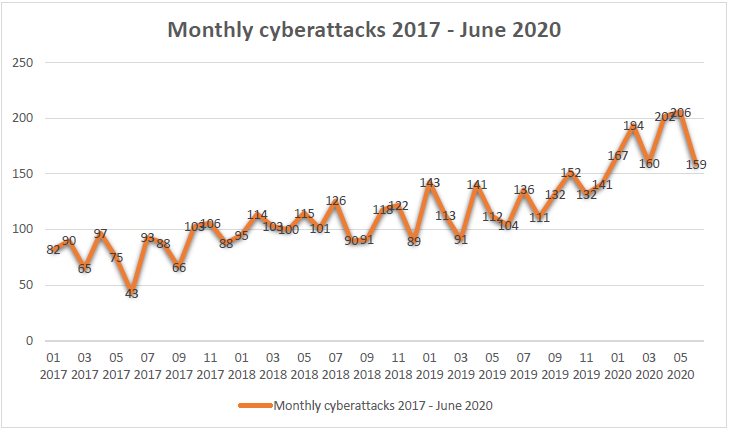
\includegraphics[width=1\textwidth]{graphics/threatscape_chart.PNG}
            \caption{Increasing number of monthly cyber attacks since 2017. Data is compiled from \cite{pt_threatscape_2018}, \cite{pt_mobile_apps_2019}, \cite{pt_threatscape_2020} and              \cite{pt_threatscape_2020q2}.}
            \label{fig:no_attacks_evolution}
        \end{figure}
		
		One of the categories of vulnerabilities that the authors of \cite{pt_mobile_apps_2019} analysed was Inter Process Communication related vulnerabilities. Inter Process Communication, abbreviated as IPC, refers to any exchange of information between two or more running processes on a computer system. In regards to Android, \cite{pt_mobile_apps_2019} also uses the term Inter Component Communication, or ICC, interchangeably with IPC. Android components are the logical building blocks of an app, and components can communicate with components, which can belong to the same app or to another app on the same device. Android components, especially if they are of the same app, can run in the same process. Therefore, IPC and ICC are not synonymous, even though they often overlap.
		
		In the study conducted in \cite{pt_mobile_apps_2019}, 29 percent of of client apps used insecure inter-process communication.
	
	\subsection{Objective}
		\label{sec:intro_objective} 
		
		In this document we present a tutorial on thesis creation and typesetting, and discuss topics such as literature surveying and proper citation. 
		
	\section{Overview}  
		\label{sec:intro_overview} 
		
		The remainder of chapter \ref{chap:intro} outlines the document structure and the key contributions of this work is organized as follows. Chapter \ref{chap:resources} reviews techniques for finding and properly citing external resources from the academic literature and online. In chapter \ref{chap:typesetting} we show examples of how to typeset different types of content, such as internal references, figures, code listings, and tables. And lastly in chapter \ref{chap:conclusion} we summarize the main contributions and key points to take away from this template.
	
	\section{Contributions} 
		\label{sec:intro_contribs} 
		
		The main contributions of this work can be seen as follows:
		
		\begin{description}	
		
			\item[$\bullet$ A LaTeX thesis template]\hfill
			
			Modify this document by adding additional TeX files for your top level content chapters. 
			
			\item[$\bullet$ A typesetting guide of useful primitive elements]\hfill
			
			Use the building blocks within this template to typeset each part of your document. Aim to use simple and reusable elements to keep your LaTeX code neat and to make your document consistently styled throughout.
			
			\item[$\bullet$ A review of how to find and cite external resources]\hfill
						
			We review techniques and resources for finding and properly citing resources from the prior academic literature and from online resources.
			
		\end{description}